\documentclass[a4paper,14pt,russian,oneside]{extarticle}
\usepackage[a4paper, text={180mm, 260mm}, left=15mm, top=15mm]{geometry}

\usepackage{fancyhdr}
\pagestyle{fancy}
\fancyhf{}
\fancyfoot[C]{\thepage}
\fancyheadoffset{0mm}
\fancyfootoffset{0mm}
\setlength{\headheight}{17pt}
\renewcommand{\headrulewidth}{0pt}
\renewcommand{\footrulewidth}{0pt}
\fancypagestyle{plain}{ 
	\fancyhf{}
	\cfoot{\thepage}}
\setcounter{page}{5}

\usepackage{cmap} % для кодировки шрифтов в pdf
\usepackage[T2A]{fontenc}
\usepackage[utf8]{inputenc}
\usepackage[russian]{babel}

\usepackage{graphicx} % для вставки картинок
\usepackage{amssymb,amsfonts,amsmath,amsthm} % математические дополнения от АМС
\usepackage{indentfirst} % отделять первую строку раздела абзацным отступом тоже
\usepackage[usenames,dvipsnames]{color} % названия цветов
\usepackage{makecell}
\usepackage{multirow} % улучшенное форматирование таблиц
\usepackage{ulem} % подчеркивания

\linespread{1.3} % полуторный интервал
\renewcommand{\rmdefault}{ftm} % Times New Roman
\frenchspacing

\usepackage{mathdots} 

\usepackage[colorlinks=true,pdfborder={0 0 0}]{hyperref}

\usepackage{float}

\renewcommand\labelenumi{\arabic{enumi}.}
\renewcommand\theenumi{\thesection.\arabic{enumi}}

\newcounter{totenum}
\setcounter{totenum}{0}
\let\Oldenumerate\enumerate
\def\enumerate{\refstepcounter{totenum}\Oldenumerate}
\newcommand{\myitem}[1]{\refstepcounter{enumi}\item[\hyperlink{#1}{\arabic{enumi}}.]}

\title{Задачи по геометрии для подготовки к Всероссийской олимпиаде школьников}
\author{Г. Р. Соснов}
\date{\today}
\begin{document}
	\maketitle
	
	\pagenumbering{arabic}
	\setcounter{page}{1}

\section{Задачи}
\begin{enumerate}
	\myitem{solution1} \hypertarget{task1}{Неравнобедренный треугольник $ABC$ вписан в окружность $\Omega$. Касательная к $\Omega$, проведенная в точке $A$ пересекает прямую $BC$ в точке $P$. Пусть $M$ и $N$ — середины сторон $AB$ и $AC$. Прямая $MN$
	пересекает $\Omega$ в точках $X$ и $Y$. Докажите, что $\angle XPA$ = $\angle YPC$.}
	\myitem{solution3} \hypertarget{task3}{Дана трапеция $ABCD$ ($AB \parallel CD$, $AB < CD$). Точки $L$ на отрезке $AB$ и $K$ на отрезке $DC$ таковы, что $\frac{AL}{LB} = \frac{DK}{KC}$. Точки $P$ и $Q$ на отрезке $KL$ таковы, что $\angle DPC = \angle ABC$ и $\angle AQB = \angle DCB$. Докажите, что $P$, $Q$, $C$ и $B$ - лежат на одной окружности.}
	\myitem{solution4} \hypertarget{task4}{Дан неравнобедренный остроугольный треугольник $ABC$. Пусть $BB_1$ — его симедиана. Луч $BB_1$ вторично пересекает описанную около треугольника $ABC$ окружность в точке $L$. Пусть $H_A$, $H_B$, $H_C$ - основания высот треугольника	$ABC$. Луч $BH_B$ вторично пересекает описанную около треугольника $ABC$ окружность в точке $T$. Докажите, что $H_A$, $H_C$, $T$, $L$ лежат на одной окружности. (Двенадцатая олимпиада по геометрии им. И.Ф.Шарыгина №12)}
	\myitem{solution6} \hypertarget{task6}{Пусть $ABC$ - треугольник с ортоцентром $H$, а $M$ — середина $BC$. Пусть $P$ и $Q$ - различные точки на окружности с диаметром $AH$, отличные от $A$, такие что $M$ лежит на прямой $PQ$. Докажите, что ортоцентр $APQ$ лежит на описанной окружности $ABC$.
	}
	\myitem{solution5} \hypertarget{task5}{Пусть $ABC$ - остроугольный разносторонний треугольник, а $M$, $N$, $P$ - середины $BC$, $CA$ и $AB$ соответственно. Пусть серединные перпендикуляры к $AB$ и $AC$ пересекают луч $AM$ в точках $D$ и $E$ соответственно, а прямые $BD$ и $CE$ пересекаются в точке $F$ внутри треугольника $ABC$. Докажите, что точки $A$, $N$, $F$ и $P$ лежат на одной окружности.}
	\myitem{solution2} \hypertarget{task2}{Пусть $ABC$ – остроугольный треугольник, в котором  $AC < BC$; $M$ – середина стороны $AB$. В описанной окружности $\Omega$ треугольника $ABC$, проведён диаметр $CC'$. Прямая $CM$ пересекает прямые $AC'$ и $BC'$ в точках $K$ и $L$ соответственно. Перпендикуляр к прямой $AC'$, проведённый через точку $K$, перпендикуляр к прямой $BC'$, проведённый через точку $L$, и прямая $AB$ образуют треугольник $\Delta$. Докажите, что описанная окружность $\omega$ треугольника $\Delta$ касается окружности $\Omega$. (Всерос 2016 10.8)}
\end{enumerate}

\section{Решения}
\begin{enumerate}
	\myitem{task1} \hypertarget{solution1}{
	Проведём прямую $l$ параллельную $BC$ через точу $A$. Пусть $l$ пересекает $BC$ в бесконечно удалённой точке $T_{\infty}$. Так как $YX \parallel BC \parallel AT_{\infty}$, то $\angle AT_{\infty}Y = \angle PT_{\infty}X$. Так как $AP$ касательная к $\Omega$, то $\angle XAP = \angle XYA$, а так как $XY \parallel AT_{\infty}$, то $\angle XAP = \angle XYA = \angle YAT_{\infty}$. Значит точки $X$ и $Y$ - изогонально сопряжены в треугольнике $T_{\infty}AP$, поэтому $\angle YPT_{\infty} = \angle XPA$ (см. рис. \ref{image1}). $\square$ 
	\begin{figure}[ht!]
		\centering
		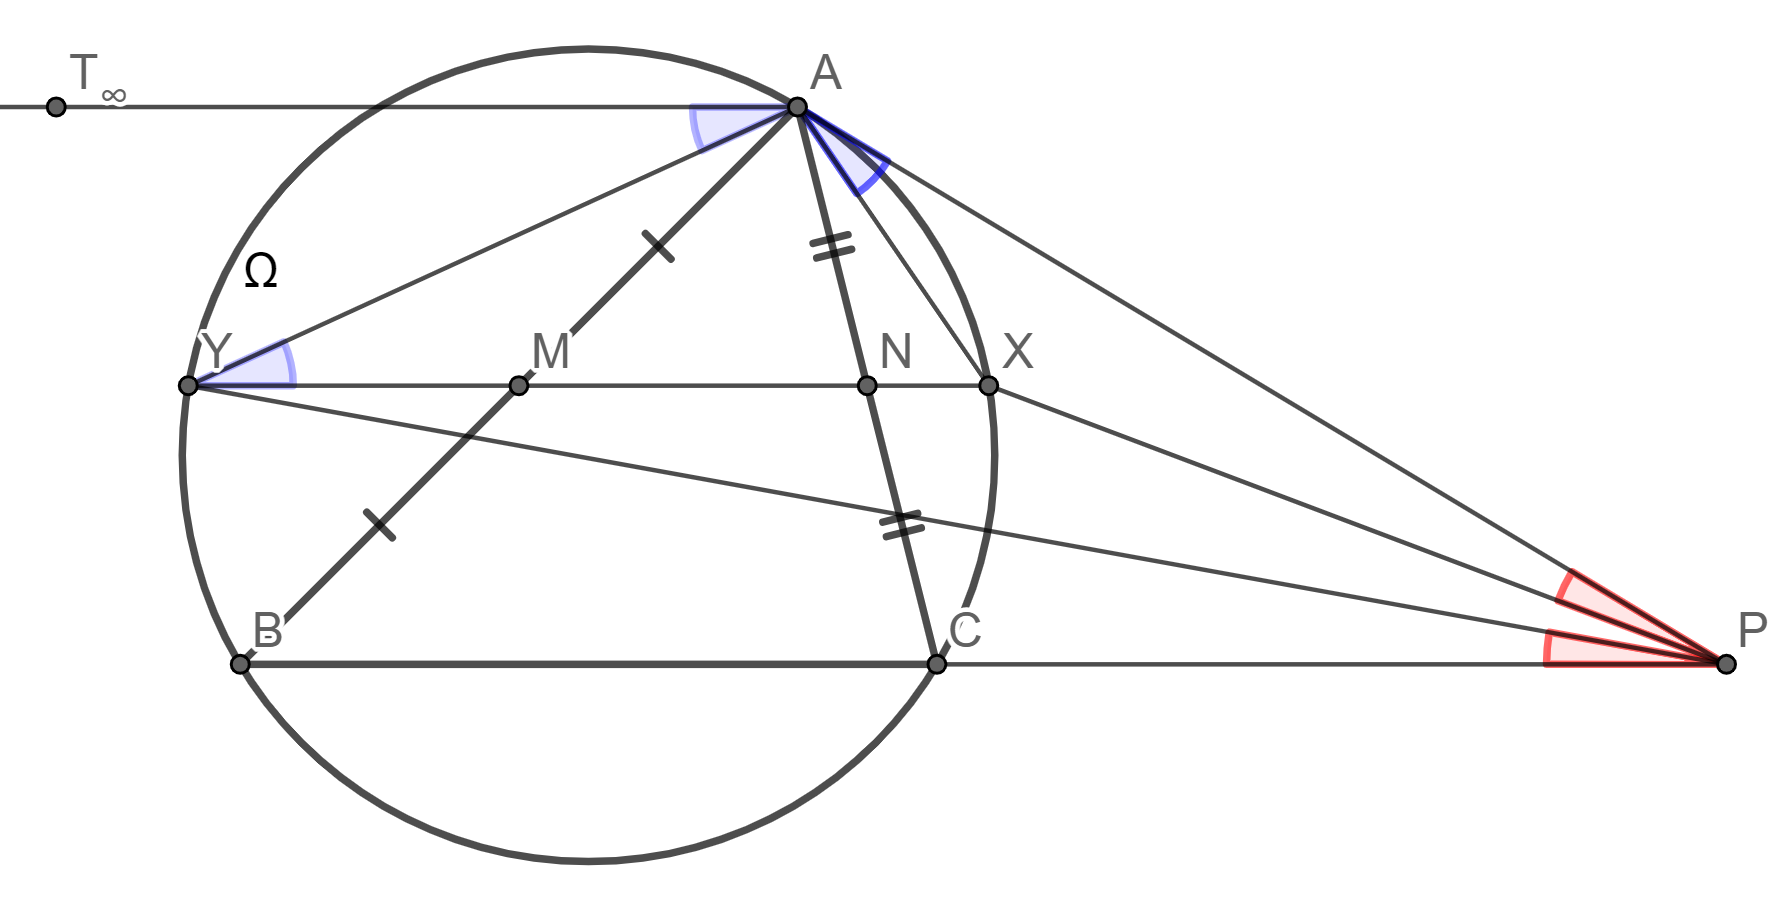
\includegraphics[width=120mm]{images/1.png}
		\caption{\label{image1}}
	\end{figure}
	}
	\myitem{task3} \hypertarget{solution3}{
	Пусть $AD$ и $BC$ пересекаются в точке $F$, тогда $K$, $L$ и $F$ - лежат на одной прямой. Действительно, сделаем гомотетию с центром в точке $F$ переводящую $AB$ в $DC$, она переводит $L$ в $K$, а значит $F$, $L$ и $K$ - лежат на одной прямой. Пусть гомотетия с центром в точке $F$, переводящая $K$ в $L$, переводит $P'$ в $P$, а $Q$ в $Q'$. Тогда $PC \parallel P'B$, $QB \parallel Q'C$, $AP'BQ$ и $DPCQ'$ - вписаны. Также описанные окружности $AP'BQ$ и $DPCQ'$ касаются $FB$ в точках $B$ и $C$ соответственно, так как $\angle AQB = \angle ABF$ и $\angle DQ'C = \angle DCF$. Так как $\angle FQ'C + \angle P'BC = \angle FQB + \angle P'BA + \angle ABC = \angle FQB + \angle AQF + \angle ABC = \angle DCB + \angle ABC = 180^{\circ}$, то $P'BCQ'$ - вписанный. Тогда $P'B$ и $Q'C$ - антипараллельны относительно $\angle KFC$, но тогда и параллельные им прямые $QB$ и $PC$ - антипараллельны относительно $\angle KFC$, то есть $PQBC$ - вписан (см. рис. \ref{image5}). $\square$
	\begin{figure}[ht!]
		\centering
		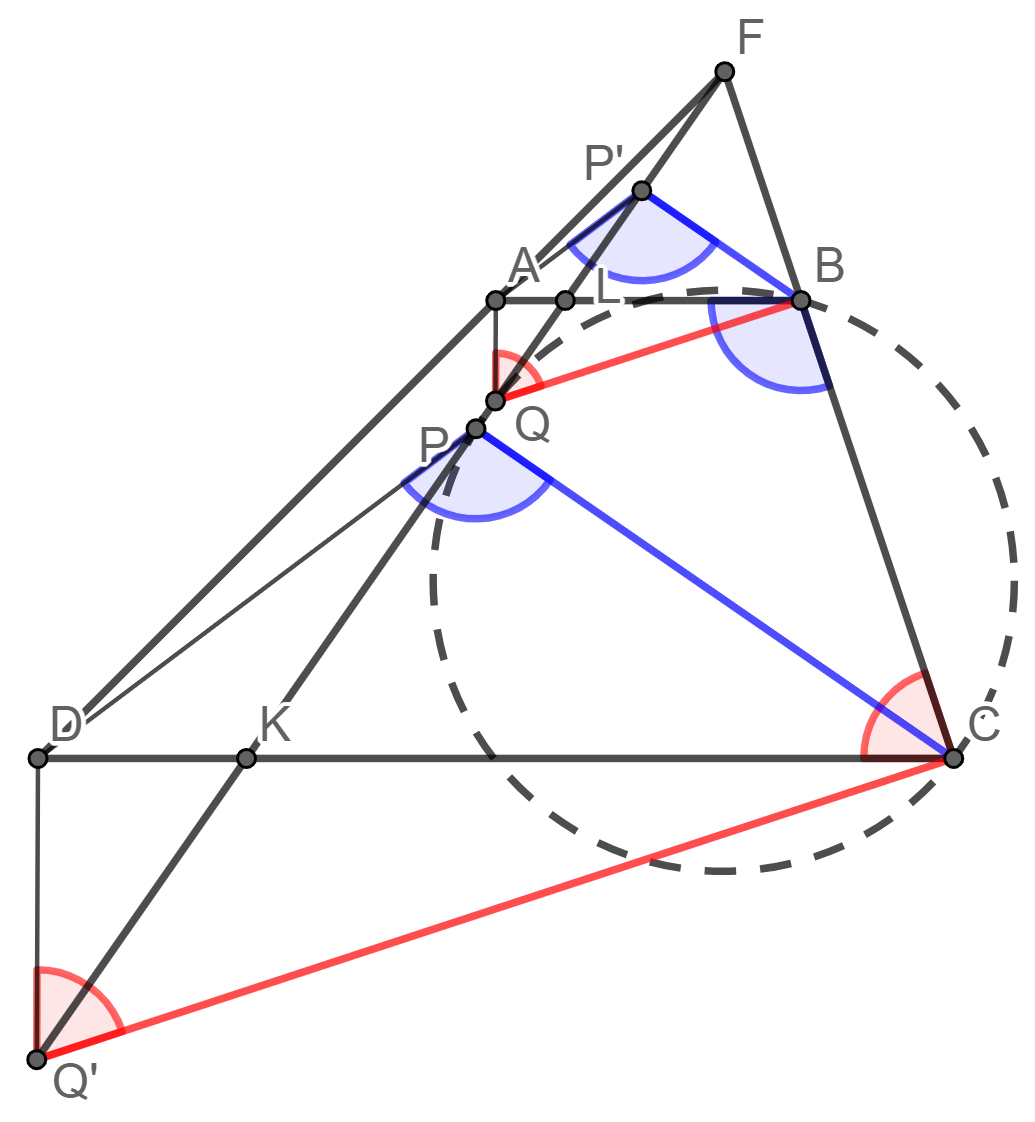
\includegraphics[width=120mm]{images/5.png}
		\caption{\label{image5}}
	\end{figure}
	}
	\myitem{task4} \hypertarget{solution4}{
	Докажем, что $AC$, $H_CH_A$ и $LT$ - пересекаются в одной точке. Пусть $LT \cap AC = P$ и $H_CH_A \cap AC = Q$. Широко известен факт, что $(A, C; H_B, Q) = -1$. Спроецируем из точки $T$ гармоническую четвёрку $A$, $C$, $B$ и $L$ на прямую $AC$, получим, что $-1 = (A, C; B, T) = (A, C; H_B, P)$, значит $P=Q$, что и требовалось доказать. Тогда, из вписанности $AH_CH_AC$ и $ACLT$: $PA \cdot PC = PH_C \cdot PH_A = PT \cdot PL$, значит $H_CH_ATL$ - вписанный (см. рис. \ref{image2}). $\square$
	\begin{figure}[ht!]
		\centering
		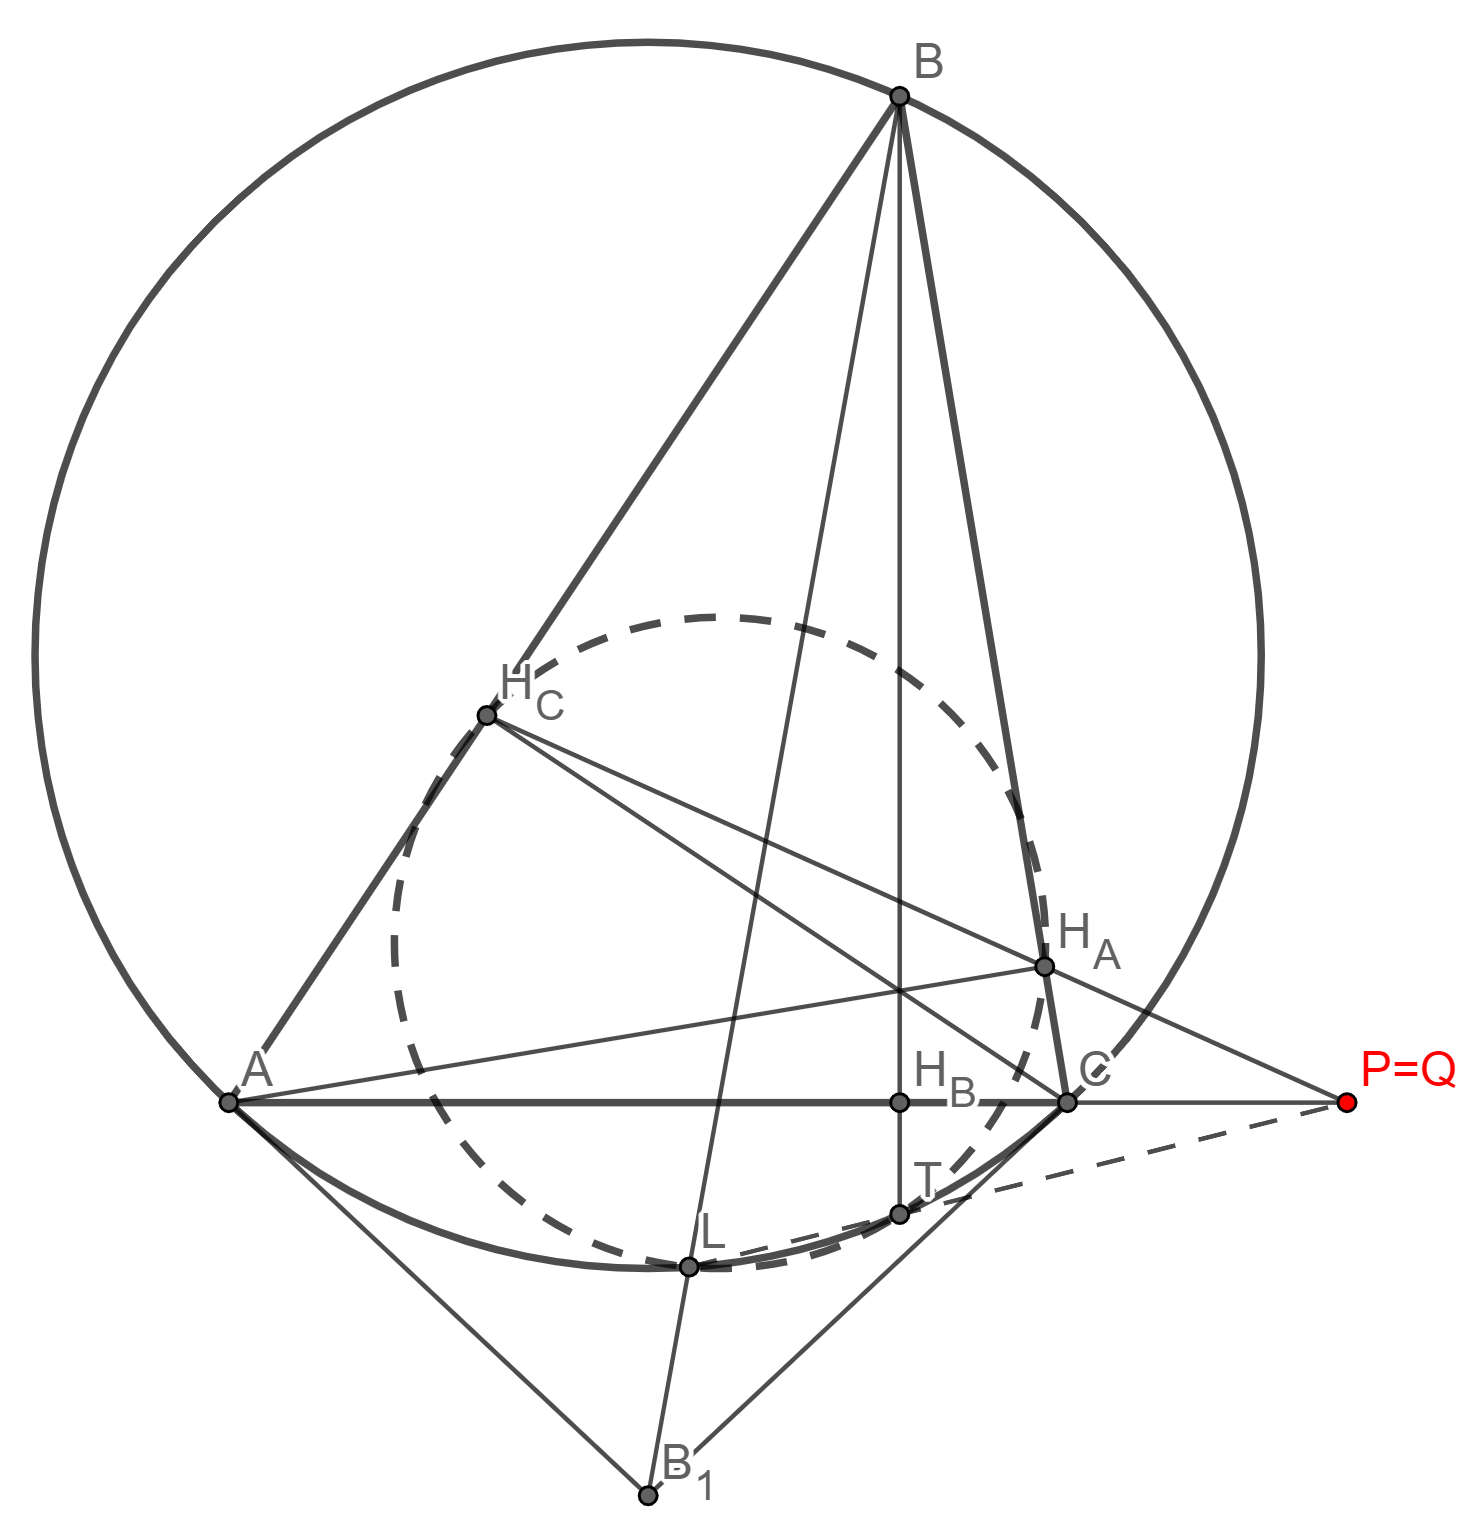
\includegraphics[width=120mm]{images/2.png}
		\caption{\label{image2}}
	\end{figure}
	}
	\myitem{task6} \hypertarget{solution6}{
	Пусть $R$ - ортоцентр $\triangle PAQ$, $K$ и $N$ - середины $AH$ и $HR$ - соответственно. Пусть $\Omega$ и $\Gamma$ - описанные окружности треугольников $ABC$ и $PAQ$, соответственно, а $\omega$ - окружность Эйлера $\triangle ABC$. Так как при центральной симметрии ортоцентра $R$ относительно $N$ он переходит в точку диаметрально противоположную точке $A$ относительно $\Gamma$ - точку $H$, то $AR \parallel KN$, тогда $KN \perp MN$. Так как $\angle KNM = 90^{\circ} = \angle KH_AM$, то $KNH_AM$ - вписан в $\omega$. Рассмотрим гомотетию с центром в точке $H$ и коэффициентом $2$, при ней $\omega$ переходит в $\Omega$, а $N$ - в $R$, то есть $R$ - лежит на $\Omega$ (см. рис. \ref{image3}). $\square$
	\begin{figure}[ht!]
		\centering
		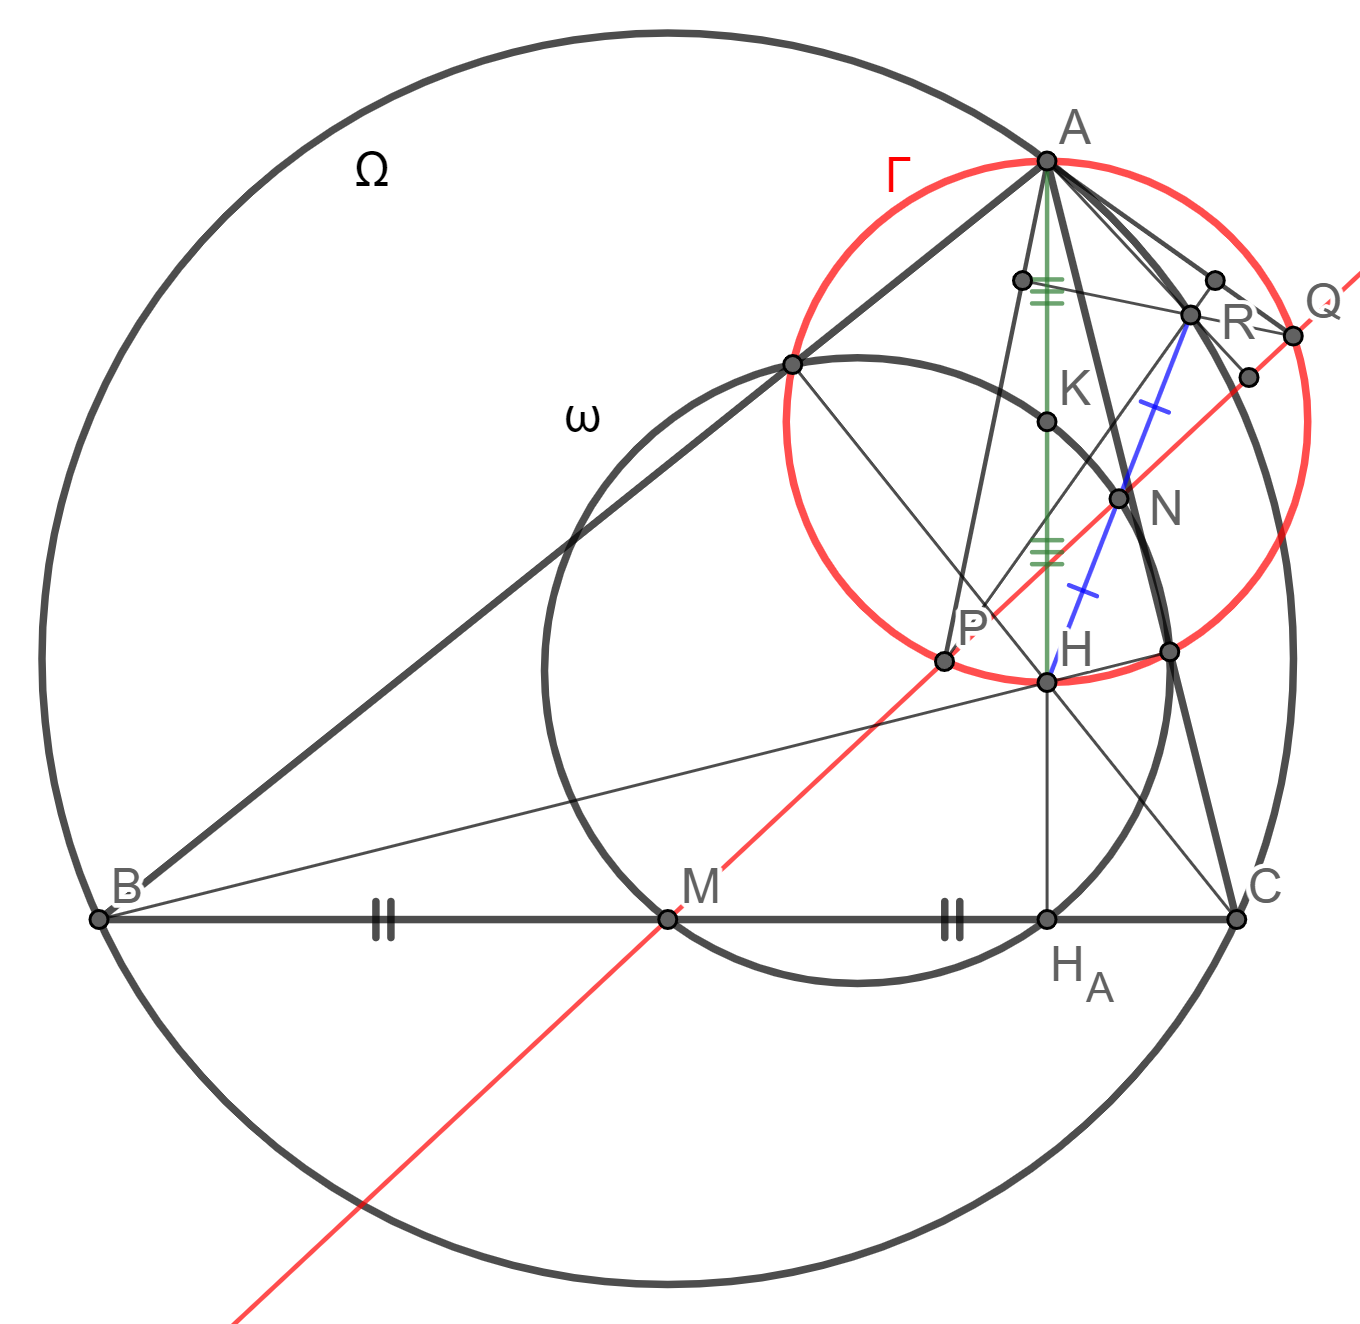
\includegraphics[width=120mm]{images/3.png}
		\caption{\label{image3}}
	\end{figure}
	}
	\myitem{task5} \hypertarget{solution5}{
	Заметим, что $F$ - точка Болтая $\triangle ABC$ вершины $A$, действительно, пусть $R$ - точка Шалтая $\triangle ABC$ вершины $A$, тогда: $\angle FBA = \angle BAR = \angle RBC$ и $\angle FCA = \angle RAC = \angle RCB$, то есть $R$ и $F$ - изогонально сопряжены, то есть $F$ - точка Болтая. Тогда $\angle FAC = \angle BAR$, $\angle FAB = \angle RAC$, то есть $\triangle BFA \sim \triangle AFC$. Рассмотрим поворотную гомотетию с центром в точке $F$ переводящую $\triangle BFA$ в $\triangle AFC$, она переводит $FP$ в $FN$, то есть $\angle PFN = \angle AFC = 180^{\circ} - \angle FAN - \angle FCA = 180^{\circ} - \angle BAC$, то есть $PFNA$ - вписанный (см. рис. \ref{image4}). $\square$
	\begin{figure}[ht!]
		\centering
		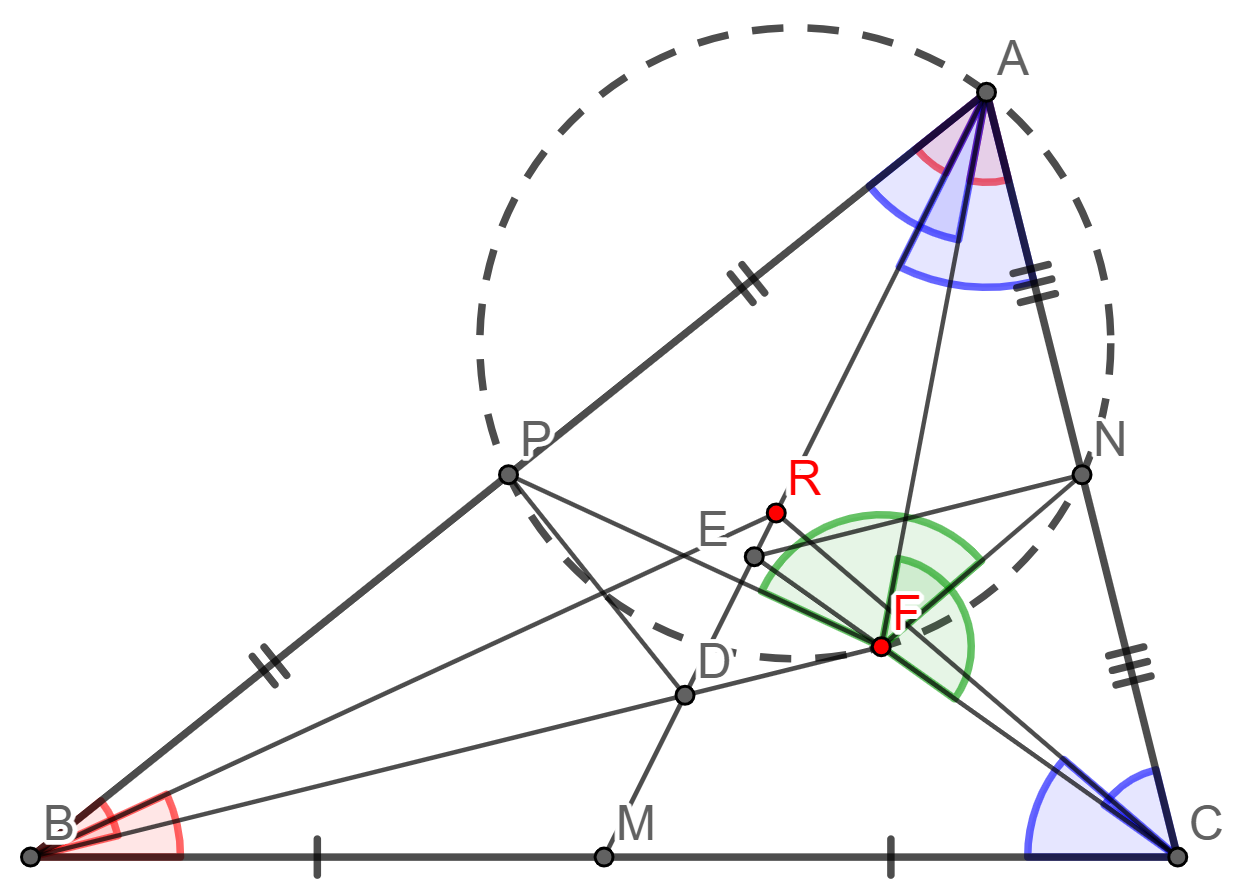
\includegraphics[width=120mm]{images/4.png}
		\caption{\label{image4}}
	\end{figure}
	}
	\myitem{task2} \hypertarget{solution2}{
	Пусть перпендикуляр к $AC'$ восстановленный из точки $K$ пересекает $AB$ в $A_1$, а перпендикуляр к $BC'$ восстановленный из точки $L$ пересекает $AB$ в $B_1$, $KA_1 \cap LB_1 = C_1$, $CM \cap \Omega = U$. Пусть треугольник $A_1B_1C_1$ вписан в $\omega$. Пусть $C'C_1$ пересекает $\Omega$ в точке $X$. Докажем, что $\omega$ и $\Omega$ касаются в точке $X$. Заметим, что $LC_1 \parallel BC$ и $KC_1 \parallel AC$, а также, что $KC_1LC'$ - вписанный, поэтому: $\angle XCA = \angle XC'A = \angle C_1LC = \angle UCB$, то есть $CX$ и $CU$ - изогонали $\angle ACB$. Получаем, что $AXUB$ - трапеция, и $XU \parallel AB$. Пусть $AU \cap BX = R$. $\angle RML = 90^{\circ} - (180^{\circ} - \angle BAC - \angle UCA) = \angle BAC + \angle ACB - \angle XBA - 90^{\circ} = 90^{\circ} - \angle XBA - \angle ABC = \angle LBR$, то есть $LBMR$ - вписанный. Получаем: $\angle RLB = 180^{\circ} - \angle RMB = 90^{\circ} = \angle C_1LB = \angle B_1LB$, то есть $LB_1$, $XB$ и $UA$ - конкурентны. Заметим, что $\angle ULB_1 = \angle XCA = \angle UAB_1$, то есть $LUB_1A$ - вписанный. Так как $R$ - лежит на радикальной оси описанных окружностей $LUB_1A$ и $ABC$, то $BR \cdot RX = AR \cdot RU = LR \cdot RB_1$, то есть $LXB_1B$ - вписанный и $\angle B_1XB = \angle B_1LB = 90^{\circ}$. $\angle C'XB_1 = \angle C'XB + \angle BXB_1 = 90^{\circ} - \angle BAC + 90^{\circ} = 180^{\circ} - \angle C_1A_1B_1$, то есть $C_1A_1B_1X$ - вписанный. Пусть прямая $l$ - касательная к $\Omega$ в точке $X$. $\angle lXC' = \angle C'BX = \angle LB_1C_1$, то есть $l$ касается $\omega$ (см. рис. \ref{image6}). $\square$
 	\begin{figure}[ht!]
		\centering
		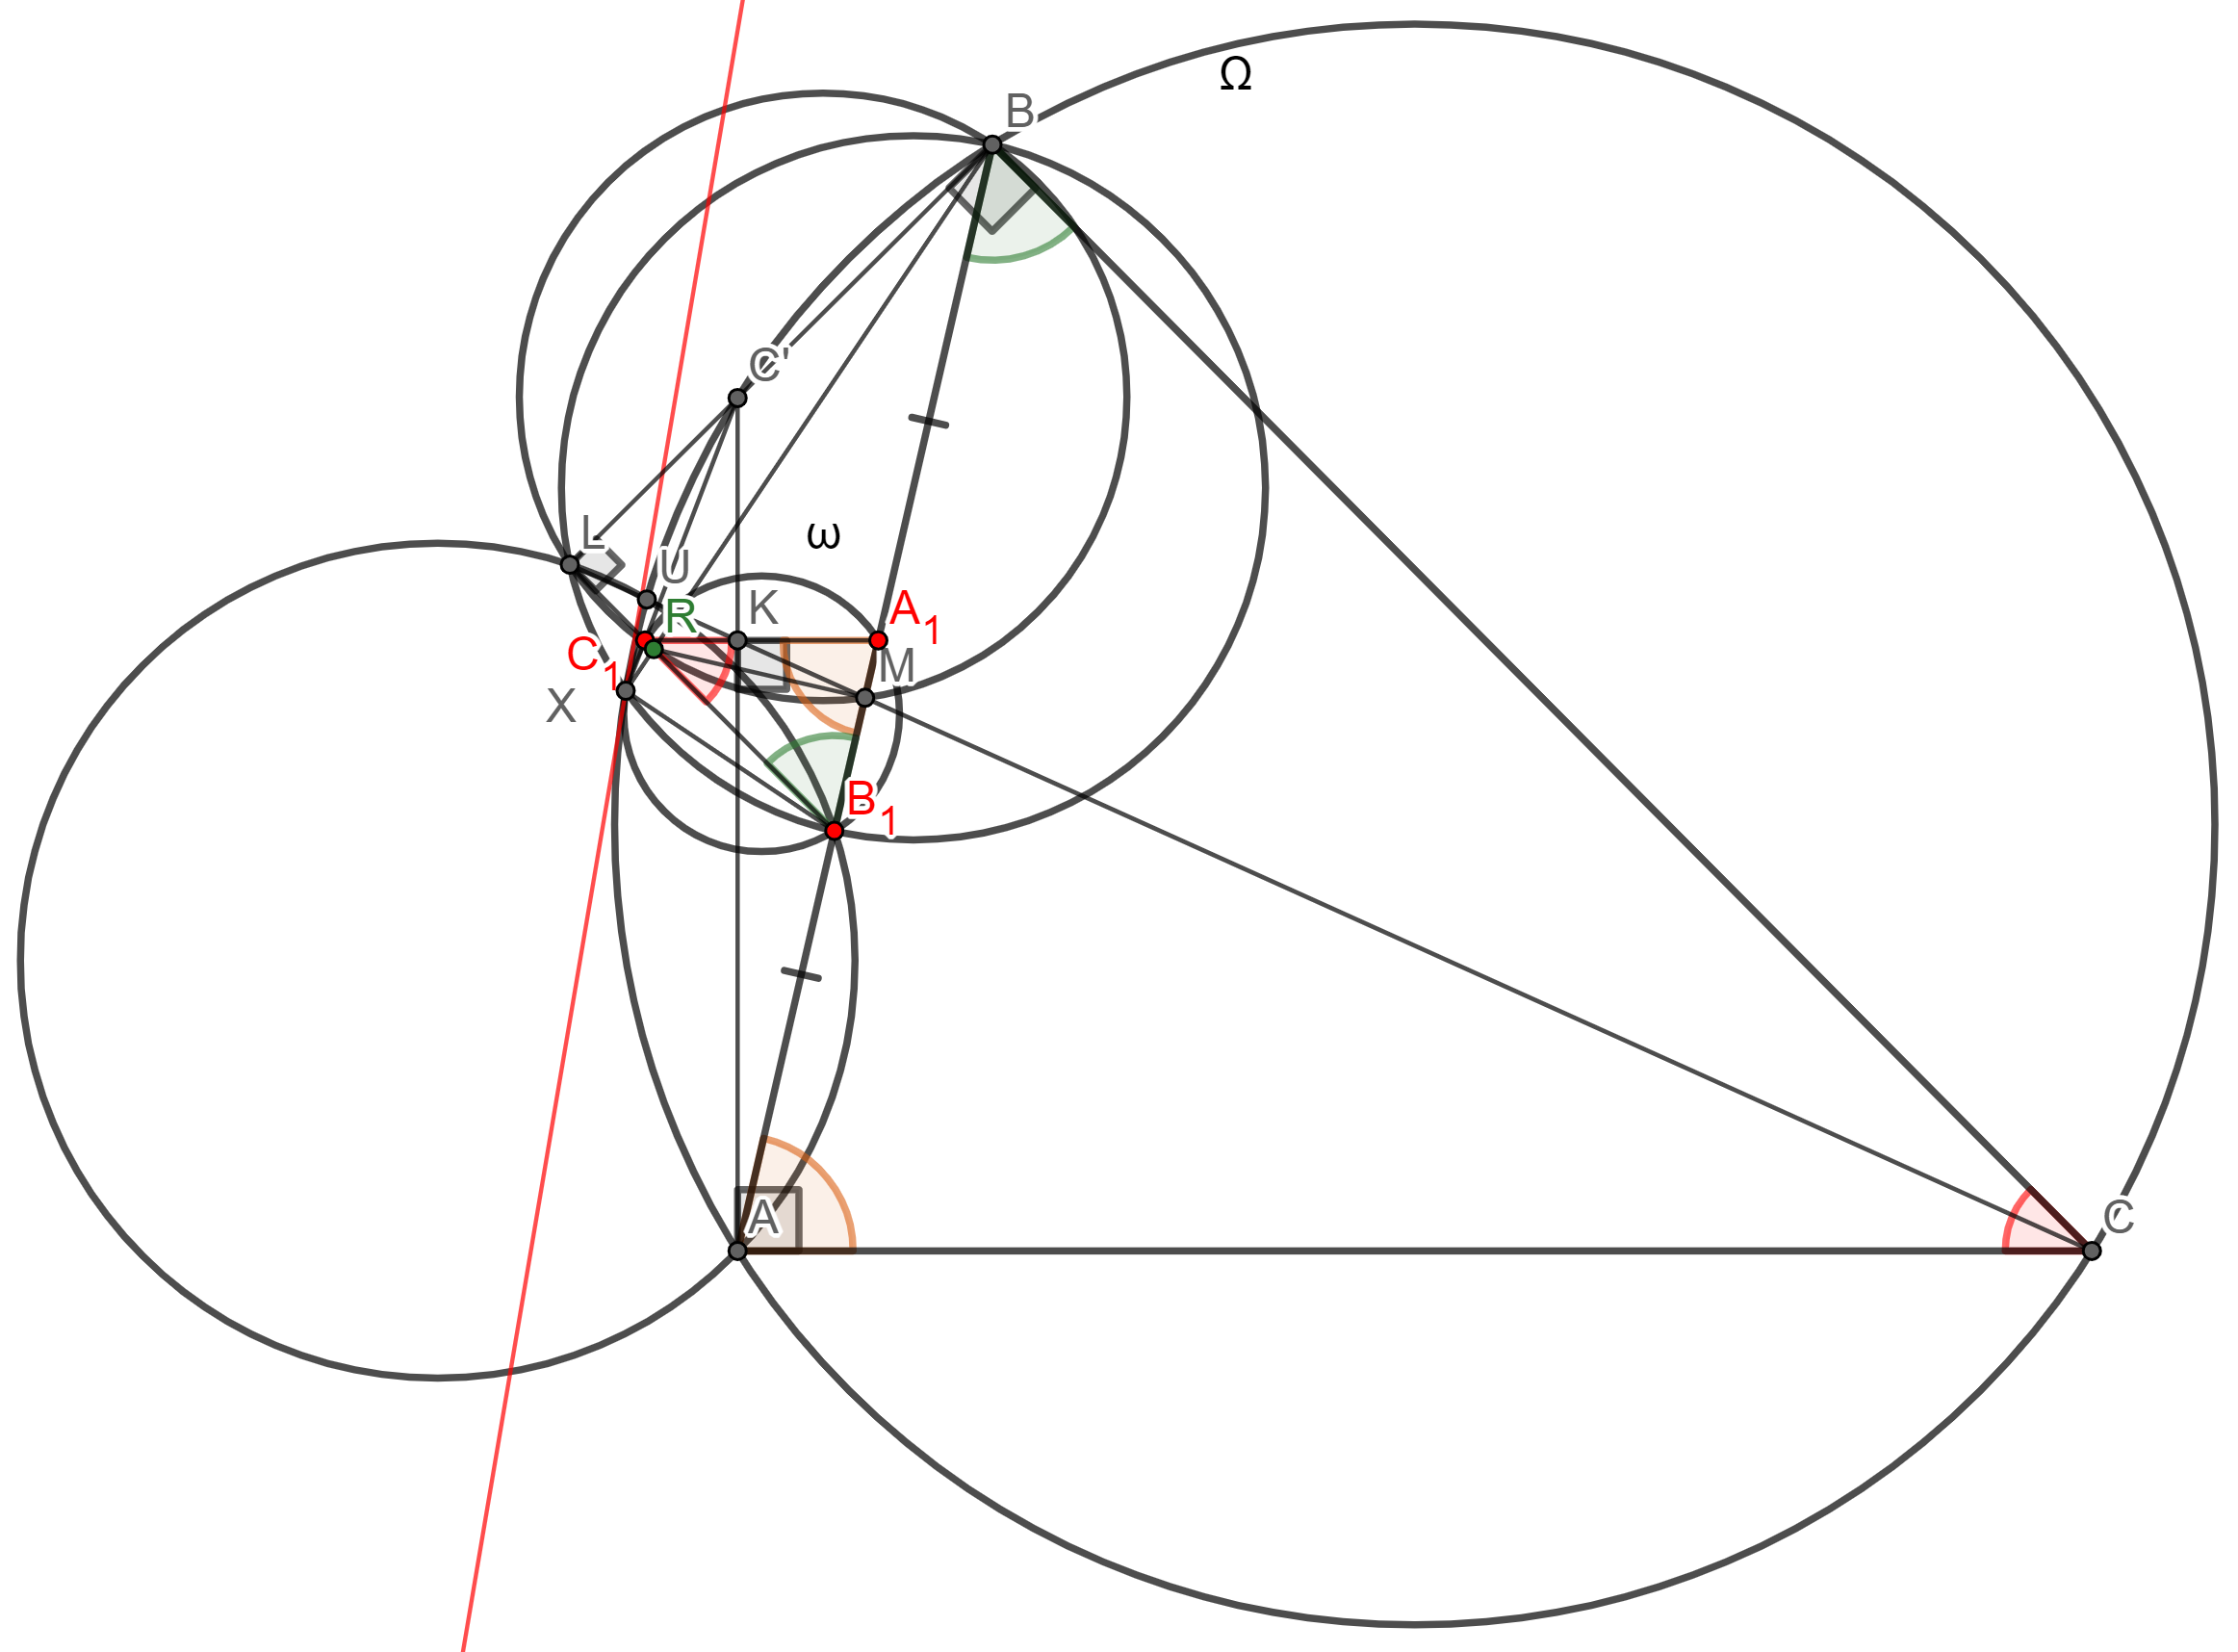
\includegraphics[width=150mm]{images/6.png}
		\caption{\label{image6}}
	\end{figure}
	}
\end{enumerate}
\end{document}